% Preamble: setup the document class and load necessary packages
\documentclass{article}
\usepackage[a4paper, includehead, left=6cm, top=2cm, right=1cm, footskip=2cm, headheight=2cm,% Set \headheight to 2cm
bottom=1.5cm]{geometry} % Set the page geometry
\usepackage{lipsum} % Dummy text package
\usepackage{etoolbox} % For programming tools
\usepackage{changepage} % To change page margins
\usepackage{dirtree} % To create directory tree structures
\usepackage[T1]{fontenc} % Font encoding
\usepackage{graphicx} % Required for including images
\usepackage{fancyhdr}
\usepackage{tikz}
\usepackage{parskip}
\usepackage{array} % for m{width} column type
\usepackage{caption} % for better spacing and customization of captions
\usepackage{makecell} % for line breaks within table cells
\usepackage{multirow} % for vertical centering in cells spanning multiple rows

% Custom maketitle command
\makeatletter
\renewcommand{\maketitle}{
    \bgroup\setlength{\parindent}{0pt}
    \begin{flushleft}
        \hspace{-5cm}\textbf{\LARGE \@title} \\ % Title
        \vspace{.4cm}
        \hspace{-5cm}\@author % Author
    \end{flushleft}\egroup
}
\makeatother

% Custom abstract environment
\renewenvironment{abstract}
    {\par\noindent\textbf{\abstractname:}\ \ignorespaces}
    {\par\medskip}

% Title and author setup
\title{Group 1: "Project Inception"}
\author{\textbf{\normalsize Alessandra Sasanelli, \normalsize Noah Schaufelberger}}

\pagestyle{fancy}
\fancyhf{}
\renewcommand{\footrulewidth}{0pt} % Eliminating footrule
\renewcommand{\headrulewidth}{0pt} 

\fancyhf[lh]{
\vspace{.6cm}
% Top rectangle
\begin{tikzpicture}[remember picture, overlay]
  \draw[fill=black] (current page.north west) rectangle ++(15cm,-0.8cm);
\end{tikzpicture}

\begin{tikzpicture}[remember picture, overlay]
  \node at (1,1.5) {
\includegraphics[width=0.3\textwidth]{press-usi-immagini-logo.png}}; 
\end{tikzpicture}

\begin{tikzpicture}[remember picture, overlay]
  \node at (9,1.8) {
    \begin{minipage}{0.2\textwidth} 
      \raggedright
      \large
      \textsf{\textbf{Università}} \\
      \textsf{\textbf{della}} \\
      \textsf{\textbf{Svizzera}} \\
      \textsf{\textbf{italiana}}
    \end{minipage}
  };
\end{tikzpicture}
}

\fancyfoot[rf]{
\vspace{.9cm}
\begin{tikzpicture}[remember picture, overlay]
  \draw[fill=black] (current page.south east) rectangle ++(-15cm,0.8cm);
\end{tikzpicture}
\begin{tikzpicture}[remember picture, overlay]
  \node at (0,.9) {
    \begin{minipage}{0.2\textwidth} 
      \textsf{\textbf{\color{white}\thepage}}
    \end{minipage}
  };
\end{tikzpicture}
}

\fancyhfoffset[l]{\dimexpr2.7in-.75in\relax}

% Begin the document content
\begin{document}	
    \maketitle % Create the title section
    
    \bigskip
    \bigskip
    
    % Abstract section
    \begin{abstract}
        This document, about the group project, contains key information about how we organized our workflow. 
        In particular, it lists all the members with their roles, the way we split the topics among the topic groups, 
        some notes about how we distributed the workload among the time we have in between each milestone.
    \end{abstract}
    
    % Horizontal rule after abstract
    \noindent\rule{\textwidth}{.5pt} 
    
    \bigskip
    
    \vspace{.2cm}
    \noindent \textbf{\large The leaders} % Section for leaders
    
    \bigskip
    
    % Table of leaders
    \noindent Here are listed the leaders:\\ \\
    \noindent \begin{tabular}{@{}ll}
        \textbf{Team Leaders} & Alessandra Sasanelli, Noah Schaufelberger\\
        \textbf{CSS Leaders} & Sebastiano Castegnero, Simone Maccario, Yhoshua Filianoti\\
        \textbf{GIT Leader} & Nicolo La Cara\\
        \textbf{Topic Leaders} & V. Levytskyi, A. Ambrogio, M. Cupryniak, X. Cai, G. Alterini\\
    \end{tabular}
    \bigskip
    
    % Section for topics and groups
    \section{Topics and groups}
    Our group is responsible for creating a website about the recent history of informatics; 
    since the time span is pretty broad, we decided to divide this topic into 5 subtopics by time spans (as shown in table \ref{tab:groups}).
    Each subtopic has been assigned to one of the five groups in which we divided our team.
    
    \noindent We have then summarized these topics to get a global overview of the contents of each part of the website:
    \begin{itemize}
    	\item \textbf{1968-1979} \\ Crucial and fundamental period for the history of Computer science. Most of technologies and inventions from this period we use in our days: the Internet, the microprocessor, UNIX operating system, C programming language, TCP/IP protocol, databases etc. Also, there were established world-known multinational corporation: Intel, AMD, Xerox PARC, Microsoft, and Apple. 
	\item \textbf{1980-1990} \\ During this time span, important technological developments that have contributed significantly to the evolution of computer technology happened. Apple listed on the stock exchange and John Backus received the Nobel Prize for Fortran. Logo programming language and Sinclair ZX80 computer introduced. IBM launched the PC. 
	\\ RISC architecture concept and introduction of SCSI and VGA interfaces. Introduction of 3.5-inch floppy disks and the computer mouse. Oracle developed its database. Created the SNMP protocol and introduced Nintendo video games. Apple launched the Macintosh. Developed standards for wireless networks. Microsoft introduced Windows 1.0, JPEG and Excel. Created the Verilog language and launched HP DeskJet printers. Windows 2.0 and NeXTSTEP operating system released. Microsoft introduced Windows 2.1 and Python was created. Windows 3.0 was released and development of Intel 80486DX2 and MIPS R4000 processors. Introduced the World Wide Web by Tim Berners-Lee. 
	\item \textbf{1991-2001} \\ Between 1990 and 2000, there was a significant surge in technological developments and the introduction of various groundbreaking tech products. These technological improvements started with the widespread adoption of personal computers with Microsoft Windows as the most dominant operating system. In the aspect of hardware, Intel released several generations of microprocessors improving speed and efficiency. On the other hand, internet became accessible to the public, while mobile phones became smaller, more affordable and widely used. In the aspect of entertainment, Sony Playstation and Nintendo 64 were introduced and E-commerce platforms, like Amazon and eBay, transformed the way people shopped. These developments laid the foundation for the digital age, shaping the way people communicate, work, and access information, and paved the way for further technological innovations in the 21st century.	\item \textbf{2002-2012} \\ This decade gave us some of the most influential companies, new developments and software we still use today. Windows XP, the release of the iPod and the launch of Mac OS X set the stage for Apple and Microsoft's dominance. The release of 3G mobile networks paved the way for the rise of mobile internet and smartphones. \\
Open-source software began to gain traction, providing an alternative development method to proprietary, corporate controlled software. WiFi revolutionised connectivity. 
Social media began its life with the founding of Facebook and Twitter. Google acquired YouTube and we saw the birth of Android, the iPhone and Google Chrome. 
	\item \textbf{2013-2023} \\ The last decade is a period of many changes in informatics. Many changes and updates. Vr technology, the beginning of advanced AI, word, excel, the progressively smaller process, the beginning of the blockchain tech and thus of cryptocurrencies, are only a few of the important advancements attained. 
    \end{itemize}
    
    \noindent\begin{table}[h!]
    \centering
    \begin{tabular}{|m{2cm}|m{3cm}|p{5cm}|m{2cm}|}
        \hline
        \textbf{Group} & \textbf{Topic leader} & \textbf{Group members} & \textbf{Assigned time span} \\ \hline
        \multirow[m]{3}{*}{Group 1}        & \multirow[m]{3}{*}{Valentyn Levytskyi}    & Robert Gomez\newline Adrian Cazar\newline Vasyl Damian & \multirow[m]{3}{*}{1968-1979} \\ \hline
        \multirow[m]{3}{*}{Group 2}        & \multirow[m]{3}{*}{Andrea Ambrogio}       & Reina Rexha\newline Nadia Kononiuk\newline Artur Lavrov & \multirow[m]{3}{*}{1980-1990} \\ \hline
        \multirow[m]{3}{*}{Group 3}        & \multirow[m]{3}{*}{Mateusz Cupryniak}          & Slovu Vlad-Stefan\newline Thomas Theodoros\newline Vleck Frantisek & \multirow[m]{3}{*}{1991-2001} \\ \hline
        \multirow[m]{3}{*}{Group 4}        & \multirow[m]{3}{*}{Xiarong Cai}           & Klaudio Musa\newline Christian Webb\newline Nicky Lokhorst & \multirow[m]{3}{*}{2002-2012} \\ \hline
        \multirow[m]{3}{*}{Group 5}        & \multirow[m]{3}{*}{Gaia Alterini}         & Xiuanlin Chen\newline Daryna Makhnonosova\newline Daniel Noshadha & \multirow[m]{3}{*}{2013-2023} \\ \hline
    \end{tabular}
    \caption{These are the groups and the assigned topics}
    \label{tab:groups}
\end{table}

    % Section for the git repository
    \clearpage
    \section{The git repository}
    Our project is being stored in a remote repository at /home/lacarn/Group\_1.
    This repository has been structured so that every group has an independent directory on which to push the files relative to that group.
    We have added one directory called "styles" on which the CSS template will be placed; this directory will be accessible by every group to work with its CSS classes. 
    The directory "docs" is needed to store every file that is not code-related; in the "how-to" folder are stored all the documentation about how to use the CSS styles and the git repository. 
    The "general" folder contains all the files related to the project development, like presentations, this "Inception" document, and many more that will be stored later. 
    The "Summaries" folder is instead used to store the summaries made by the group topics at the very early stage of the project ideation.
    
    \bigskip
    
    % Directory tree
    \dirtree{%
        .1 Group\_1.
        .2 styles.
        .2 docs.
        .3 how-to.
        .3 general.
        .3 Summaries.
        .2 sg1.
        .3 html.
        .3 css.
        .3 resources.
        .2 sg2.
        .3 html.
        .3 css.
        .3 resources.
        .2 sg3.
        .3 html.
        .3 css.
        .3 resources.
        .2 sg4.
        .3 html.
        .3 css.
        .3 resources.
        .2 sg5.
        .3 html.
        .3 css.
        .3 resources.
    }
    
    \pagebreak
    
    \section{Our schedule}
    We organised our work as shown in figure \ref{fig:schedule}. 
    
    The css leaders already started with the general planning of the site style; this will be then refined with a brainstorming session to group ideas for the site appearance (on the 7th of November 2023); this will be an important session to get everybody's contribution to the site as a whole. On the 8th of November, after the Inception, in which we'll have the confirmation or not to start our project, we will begin with the writing of the single pages. During this phase, every group leader will be encouraged to divide between the members the creation of the pages for that topic. Once every body will be assigned with a part, they'll begin with the effective writing of the page. To get in touch with the work that is getting done week by week, we'll have every Friday a meeting session with the group leaders. 
    
    We've planned a first correcting sessions by the time everybody will have created at least 2 pages; this way, in case something is not looking as it should or if any other kind of problem is encountered, we can solve them with ease. After this phase, on the 15th there will be the css delivery; here, the css team must be done with the general template for the whole site. 
    
    The last phase is the most crucial one; everybody must be done with its individual work so that we can have a final revision of the work. This final delivery (planned for the 17th of November) is intended to let us, team leaders, have time to review all of the work that has been done, to correct the code, and to eventually add the missing part in case some people didn't work as intended. 
    
    
    \pagebreak
    \vspace{-3cm} 
    \begin{figure}
    	\centering
    	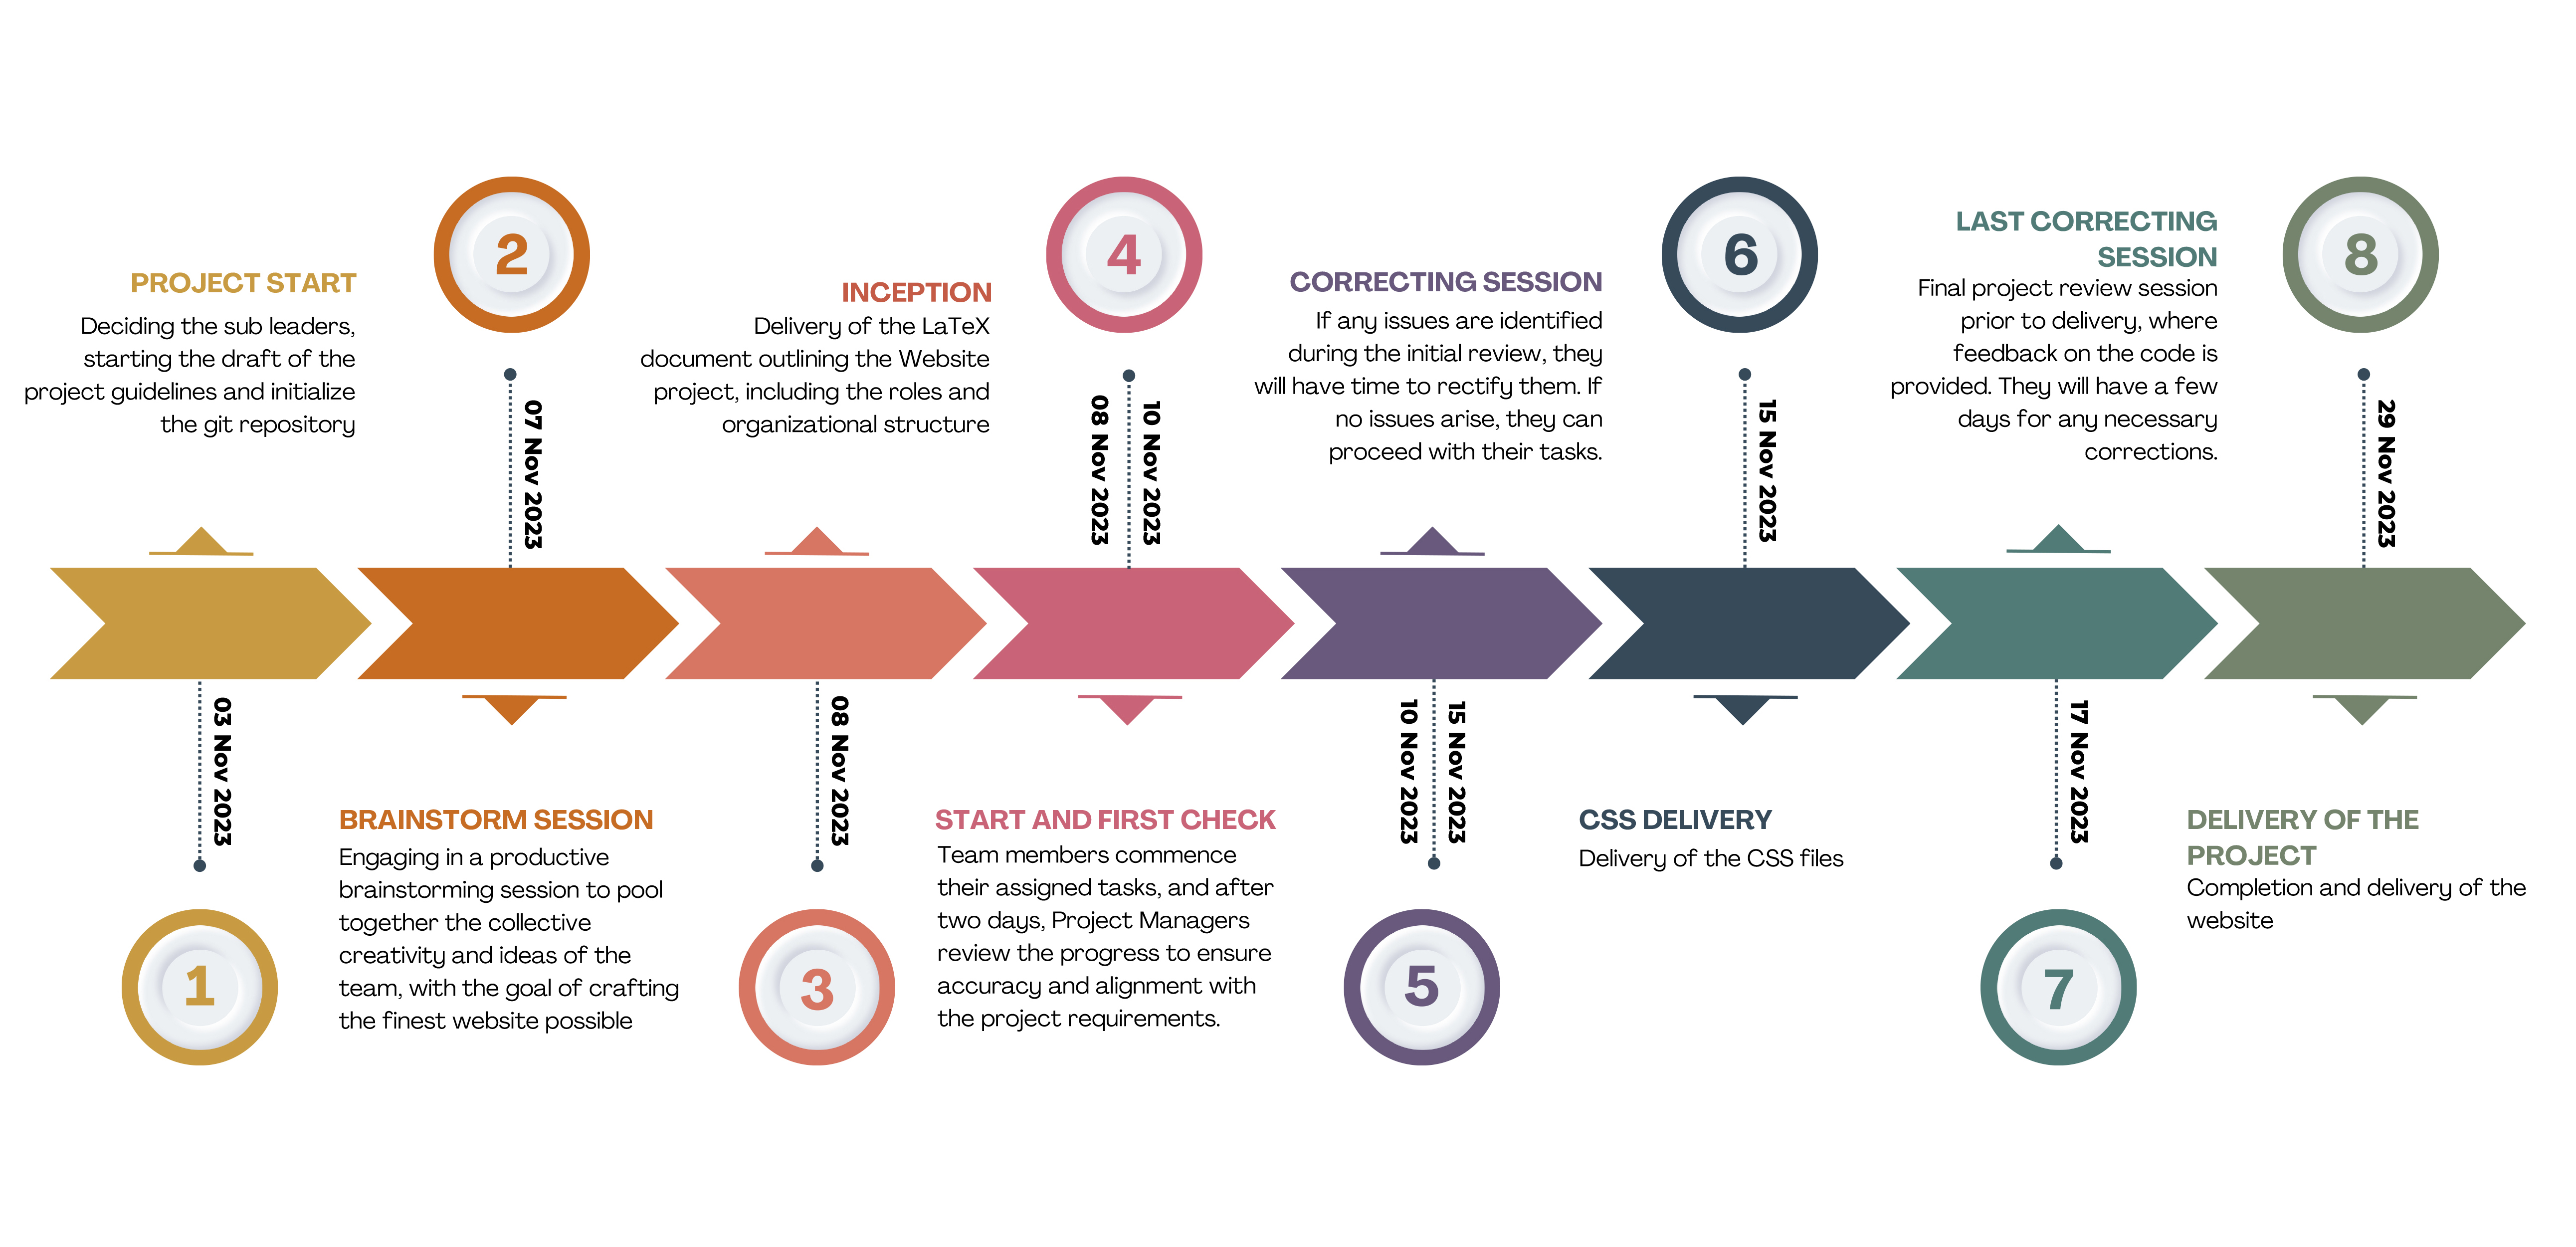
\includegraphics[width=10cm, height=20cm]{timeline.jpg}
	\caption{Our schedule timeline}
	\label{fig:schedule}
    \end{figure}

% End the document content
\end{document}
